% -- Encoding UTF-8 without BOM
% -- XeLaTeX => PDF (BIBER)

\documentclass[]{cv-style}          % Add 'print' as an option into the square bracket to remove colours from this template for printing. 

\sethyphenation[variant=british]{english}{} % Add words between the {} to avoid them to be cut 

\usepackage{hyperref}
\hypersetup{
    colorlinks=true,
    linkcolor=cyan,
    filecolor=cyan,      
    urlcolor=cyan,
}

\begin{document}

\header{}{Emily Quinn Finney}           % Your name
%\lastupdated

%----------------------------------------------------------------------------------------
%	WORK EXPERIENCE SECTION
%----------------------------------------------------------------------------------------

\section{Data/Software Development Experience}

\begin{entrylist}
%------------------------------------------------

\entry
  {2017}
  {Participant}
  {New York, NY}
  {\jobtitle{Recurse Center} 
  \begin{itemize}
    \item Accepted to a three-month self-directed \href{https://www.recurse.com/}{program} for software developers.
    \item Built an asynchronous breadth-first-search \href{https://github.com/eqfinney/web-scraping}{web crawler} in Python using the asyncio and Beautiful Soup packages.
    \item Implemented a content-based \href{https://github.com/eqfinney/recommender-system}{recommender system} using data obtained from Charity Navigator.
    \item Wrote a \href{https://eqfdatadiary.com/}{technical blog} to solidify my understanding of these projects.\\
  \end{itemize}}
\entry
  {2015-2017}
  {Graduate Research Associate}
  {Davis, CA}
  {\jobtitle{University of California, Davis} 
  \begin{itemize}
    \item Trained high-dimensional models of galaxy cluster structure using MCMC and gradient descent algorithms. 
    \item Built a data pipeline for analyses using tools from the SciPy stack. 
    \item Refactored image smoothing code, leading to 100x speedup.
    \item Wrote a peer-reviewed journal article detailing results.\\
  \end{itemize}}
\entry
  {2013}
  {Undergraduate Senior Thesis}
  {Claremont, CA}
  {\jobtitle{Scripps College} 
  \begin{itemize}
    \item Implemented Bayesian methods to improve models of galaxy cluster mergers. 
    \item Constrained galaxy cluster collision parameters by 70-85\%.
    \item Visualized data and communicated analysis and results in a \href{https://github.com/eqfinney/thesis-2013/blob/master/EQF_thesis.pdf}{paper}.
    \item Selected to present research at Scripps College Capstone Day.\\
  \end{itemize}}
\entry
  {2012, 2013}
  {Undergraduate Research Internships}
  {Davis, CA; La Serena, Chile}
  {\jobtitle{University of California, Davis; Cerro Tololo Inter-American Observatory}
  \begin{itemize}
    \item Classified spectral data and fit lines to redshifts to improve detection of high-mass galaxy clusters.
    \item Cleaned gigabytes of astronomical data using bash scripting.
    \item Conducted hypothesis testing on a set of galaxy ellipticity data.\\
  \end{itemize}}

%------------------------------------------------

\end{entrylist}


%----------------------------------------------------------------------------------------
%	SKILLS SECTION
%----------------------------------------------------------------------------------------

\section{Teaching Experience}

\begin{entrylist}
%------------------------------------------------

\entry
  {2017}
  {Tutorial Speaker, Teen Track}
  {Davis, CA}
  {\jobtitle{SciPy 2017 Conference} 
  \begin{itemize}
    \item Led 22 students ages 12-18 in an exploration of the SciPy stack.
    \item Created a set of interactive \href{https://github.com/eqfinney/SciPy}{Jupyter notebooks} to facilitate students' learning.\\
  \end{itemize}}
\entry
  {2017}
  {Elementary Math/Science Teacher}
  {Davis, CA}
  {\jobtitle{Peregrine School} 
  \begin{itemize}
    \item Organized activities and commmunicated material to a class of $\sim$20 students.
    \item Designed and implemented project-based lesson plans.\\
  \end{itemize}}

%------------------------------------------------

\end{entrylist}
  
%\entry
%  {2014-2016}
%  {Physics Teaching Assistant}
%  {Davis, CA}
%  {\jobtitle{University of California, Davis}
%  \begin{itemize}
%    \item Taught physics discussion/labs for 40-60 students each academic quarter.
%    \item Responsible for weekly office hours, grading, and proctoring exams.\\
%  \end{itemize}}
%\entry
%  {2012-2014}
%  {Physics and Computer Science Tutor/Grader}
%  {Claremont, CA}
%  {\jobtitle{Scripps College; Harvey Mudd College}
%  \begin{itemize}
%    \item One-on-one tutoring in physics and computer science concepts.\\
%  \end{itemize}}
%\entry
%  {Summers}
%  {Camp Director}
%  {Davis, CA; Reno, NV; Plymouth, MA}
%  {\jobtitle{The Peregrine School; Great Basin Institute; Camp Clark YMCA}
%  \begin{itemize}
%    \item Designed and implemented physics, ecology, and computer programming oriented curricula for students ages 4-16.\\
%  \end{itemize}}
%------------------------------------------------

%----------------------------------------------------------------------------------------
%	EDUCATION SECTION
%----------------------------------------------------------------------------------------

\section{Education}

\begin{entrylist}
%------------------------------------------------
\entry
{2014--2017}
{Master's of Science, Physics}
{Davis, CA}
{\jobtitle{University of California, Davis}}

{\vspace{-0.2cm}}
\end{entrylist}
%------------------------------------------------
\begin{entrylist}
\entry
{2010--2014}
{Bachelor's of Arts, Physics}
{Claremont, CA}
{\jobtitle{Scripps College}}
\end{entrylist}

%----------------------------------------------------------------------------------------
%	INTERESTS SECTION
%----------------------------------------------------------------------------------------

\section{Other Skills and Interests}
  \vspace{-0.2cm}

  \textbf{Professional} \hspace{0.05cm} Machine learning, tidy data, image analysis, data-driven education. \\
  \textbf{Personal} \hspace{0.57cm} Hiking, child development, spiders, theology, singing.
  
%----------------------------------------------------------------------------------------

%----------------------------------------------------------------------------------------
%	SIDEBAR SECTION  -- In the aside, each new line forces a line break
%----------------------------------------------------------------------------------------

\begin{aside}
%
\section{Software}
\textbf{Python}
%{\color{red} $\varheartsuit$} 
NumPy\\ SciPy\\ Pandas\\ matplotlib
%\LaTeX{}
\textbf{Unix/Linux}
bash scripting
Git
\textbf{Software Design}
OOP
Testing frameworks
C data types
\textbf{R}
tidyverse enthusiast
\textbf{Other Languages}
Java\\ MATLAB\\ SQL\\ \LaTeX
%
\section{Practical Statistics}
\textbf{Bayesian Methods}
Bayes' Theorem
MCMC
\textbf{Statistical Inference}
Random variables
Hypothesis testing
Regression
Experimental design
\textbf{Machine Learning}
Gradient descent
Clustering algorithms
\textbf{Mathematics}
Linear algebra
Multivariate calculus
%
\section{Photo}
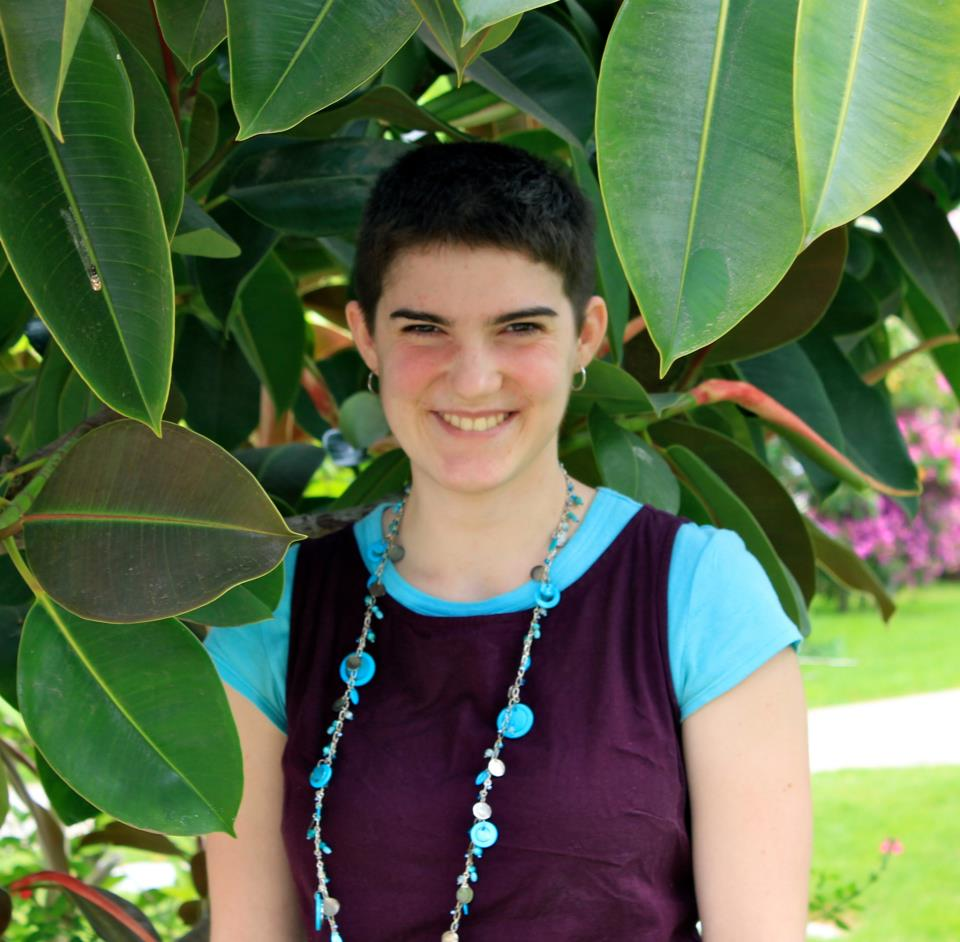
\includegraphics[width=3.6cm,height=3.6cm]{headshot.jpg}
%
\section{Contact}
\fontsize{8}{10}\selectfont
549 Commercial Ave Apt. 6\\ South San Francisco, CA \\\hspace{0.5cm}94080
%
eqfinney@ucdavis.edu
%
(339) 933-3936
%
\href{https://twitter.com/eqfinney}{@eqfinney}
%
\href{https://eqfdatadiary.com/}{eqfdatadiary.com}
%
\href{https://github.com/eqfinney}{github.com/eqfinney}
%
\href{linkedin.com/in/emily-quinn-finney}{linkedin.com/in/\\\hspace{0.5cm}emily-quinn-finney}
\end{aside}

\end{document}
